\documentclass{standalone}
\begin{document}

Previously, in our approach the Humanoid robot had to insert the
wrench into the shaft and rotation of 360$^{\circ}$ was achieved
by moving the arm along the constraint space of solvable inverse
kinematics (IK). Due to joint limitations at certain movements, IK may
not be solved for some estimated trajectories. Initially, we rotated
the wrench at $4$ intervals, whereby an interval rotation was
$90^{\circ}$. A drawback of this strategy is the time requirement to
complete the task. As a consequence, we designed a new
gripper that use the servo motor attachment. With this design the
robot can directly accomplish the rotation of $5Nm$ torque task
without having to solve multiple IK's.

%% The last gripper in task 2 our humanoid robot have to fit the wrench
%% into the shaft and rotate $360$ degrees by move the arm and solve the
%% inverse kinematics. However, sometimes(usually) the inverse kinematics
%% can not be solved due to the limitation of the arm. In the first
%% report we attempt to rotate the wrench $4$ times with $90$ degrees
%% each time. This is very time consuming and now we designed a new
%% gripper that use the servo motor attached to the gripper which can
%% directly robot $360$ degrees and capable of the torque $5Nm$. 


Figure \ref{gripper} illustrates the new gripper which consists of a
servo motor and a magnetic attachment. We used a Dynamixel MX-106
servo motor which has a high stall torque
of $8.4Nm$. With a torque load of $5Nm$, it can rotate at a speed of
more than $10 rpm$ thus saves alot of time.
To pick and align the wrench into the shaft, the gripper is equipped
with a spring attachment. When the wrench is picked by the robot, the
spring push the central stick inside the ring end of the wrench to
ensure perfect alignment. The ring end of the wrench is used to
manipulate the shaft. To align the wrench to the shaft, only the
central stick needs to be aligned to the shaft. After alignment, the
gripper is pushed against the shaft which will result in the spring to
compress and the ring end of the wrench pushed into the shaft as shown
on the right in Fig.\ref{gripper}. The shaft is then easily rotated
using the Dynamixel motor.

%% FUTURE WORK
%% <<<<<<<<<<<<<<<<<
%% We need more experiments to validate the feasibility of
%% this gripper and then we can decide whether to equip this kind of
%% gripper in the final or not.
%% >>>>>>>>>>>>>>>>>>>>

 \begin{figure}%[hb]
    \begin{center}
    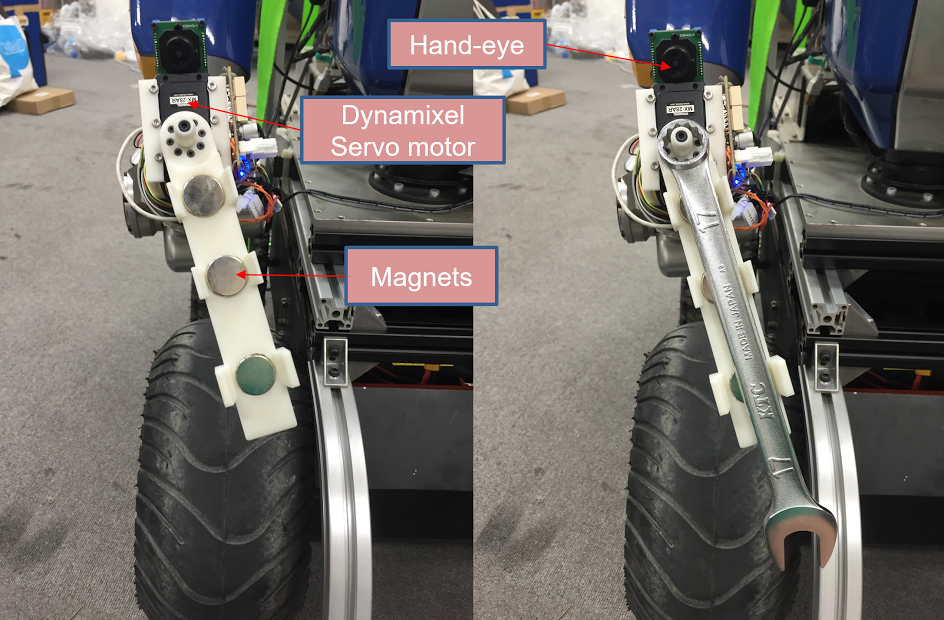
\includegraphics[keepaspectratio=true, width=1\linewidth,
      height=0.3\textheight]{sections//task2//images//gripper.png}
      \end{center}
    \caption{New Gripper Design}
    \label{gripper}
 \end{figure}

\end{document}
